\documentclass[../main.tex]{subfiles}
\addbibresource{../bibfile.bib}

\begin{document}

\chapter{Metodologie utilizzate}
\label{chap:oth}
Questo capitolo è dedicato all'esposizione delle diverse metodologie statiche e dinamiche alla base delle tecniche di analisi rese disponibili dalla piattaforma.
In particolare, verranno illustrati i concetti teorici alla loro base e verranno forniti esempi per illustrare il funzionamento di alcune tecniche su casi concreti.
\section{Control Flow Graph (CFG)}
Considerare adeguatamente il flusso di controllo di un programma, cioè quali istruzioni vengono eseguite dato un certo input, è fondamentale per effettuare un'analisi di sicurezza accurata. Risulterebbe infatti inutile segnalare
una problematica di sicurezza data da un segmento irraggiungibile del codice di un programma.
Possiamo notare che quando vi sono due istruzioni in sequenza, l'esecuzione della prima implica l'esecuzione della seconda. 
Chiamiamo quindi \textit{basic block} una \textbf{sequenza massimale contigua di statement del programma}.
Per rappresentare in modo esaustivo tutti i possibili cammini di esecuzione che un programma può intraprendere, possiamo ricorrere ad una struttura a grafo chiamata \textbf{Control-Flow Graph} (CFG).
Dato un programma $P$, un CFG per $P$ è un grafo $G$ \textbf{diretto e orientato} dove:
\begin{itemize}
    \item I nodi di $G$ sono i basic block del programma
    \item Gli archi di $G$ connettono i basic block che sono in una relazione di sequenza (uno segue l'altro). Gli archi che derivano da una scelta condizionale (es. \textit{if}) sono etichettati con "true" e "false"
\end{itemize}
Durante la costruzione di un CFG, è importante gestire correttamente le istruzioni che modificano il flusso di controllo, come \textit{if} e \textit{while}:
\begin{itemize}
    \item \textbf{If}: Il controllo condizionale termina il basic block a cui appartiene lo statement immediatamente precedente. Due archi etichettati "true" e "false" connettono il basic block contenente la condizione rispettivamente ai rami \textit{then} e \textit{else}.
    Gli archi uscenti dai basic block dei due rami sono diretti verso il basic block contenente gli statement che seguono l'intera struttura dell'istruzione condizionale.
    \item \textbf{While}: Questo statement crea un \textbf{basic block a se stante}, il quale avrà due archi uscenti etichettati rispettivamente "true", verso il basic block del corpo del ciclo, e "false", verso il basic block degli statement successivi al ciclo.
\end{itemize}
\newpage \noindent
Supponiamo, per esempio, di avere il seguente programma e di volerne costruire il CFG:
\lstinputlisting[language=C, caption = Un programma in C che calcola il massimo numero in un array di cinque elementi, firstline = 3]{../code_examples/exemple1.c}
\begin{figure}[H]
    \centering
    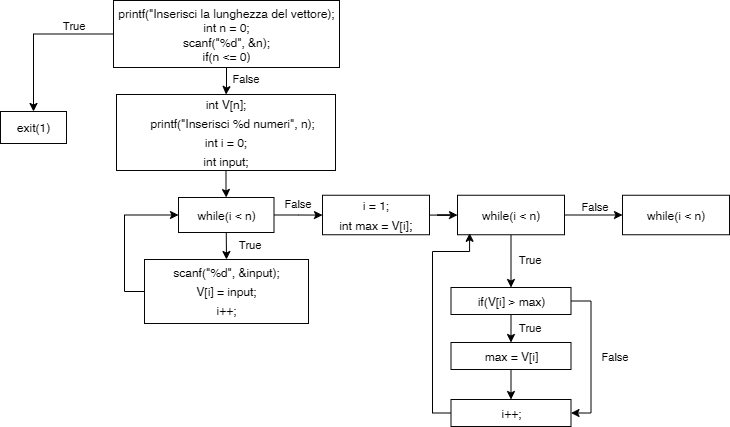
\includegraphics[width = 1\linewidth]{../images/CFG.drawio.png}
    \centering
    \caption{CFG del programma illustrato nel listing 3.1}
\end{figure}
\section{Data Dependence Graph (DDG)}
Quando si effettua l'analisi di un programma, oltre alla rappresentazione del flusso di controllo tramite CFG, risulta a volte utile tracciare le relazioni di dipendenza che sussistono tra le istruzioni del programma.
Questo tipo di analisi permette infatti di individuare l'origine e l'utilizzo di variabili potenzialmente inquinate da dati malevoli. Per rappresentare queste relazioni possiamo usare una struttura a grafo che prende il nome
di \textbf{Data-Dependence Graph} (DDG). Possiamo derivare un DGG direttamente dal CFG di un programma, tuttavia dobbiamo avere prima una definizione chiara di \textbf{dipendenza} fra gli statement; una possibile definizione è quella che prende il nome di \textbf{dipendenza per flusso} (flow-dependence) \cite{DDG}:
Sia $G = (V, E)$ il CFG per un programma $P$ e siano $DEF(i)$ e $REF(i)$ gli insiemi che denotano rispettivamente le variabili definite e referenziate in un nodo $i \in V$ del CFG.
Allora, un nodo $j \in V$ è \textbf{dipendente} dal nodo $i$ rispetto ad una certa variabile se e solo se esiste una variabile $x$ tale che:
\begin{enumerate}
    \item $x \in DEF(i)$
    \item $x \in REF(j)$
    \item Esiste un cammino da $i$ a $j$ senza definizioni intermedie della variabile $x$ (es. Altri assegnamenti ad $x$ ecc...)
\end{enumerate} 
Applicando quindi la definizione di dipendenza data, sussiste una relazione di dipendenza tra due statement $S1$ e $S2$ se:
\begin{enumerate}
    \item $S1$ definisce una variabile $x$
    \item $S2$ contiene un riferimento ad $x$
    \item Esiste un cammino da $S1$ a $S2$ dove $x$ non viene ridefinita. Ciò significa che la definizione di $x$ data in $S1$ viene utilizzata in $S2$.  
\end{enumerate}
Quindi, un DDG $D$ per un programma $P$ è un grafo \textbf{diretto e orientato} dove:
\begin{itemize}
    \item I nodi di $D$ rappresentano gli statement del programma
    \item Gli archi di $D$ rappresentano le relazioni di dipendenza tra due statement
\end{itemize}
Supponiamo, per esempio, di avere il seguente programma e di volerne costruire il DDG:
\lstinputlisting[language=C, caption = Un programma in C che calcola il prezzo di un prodotto. Esempio proventiente da \cite{DDG}, firstline = 2]{../code_examples/example2.c}
\begin{figure}[H]
    \centering
    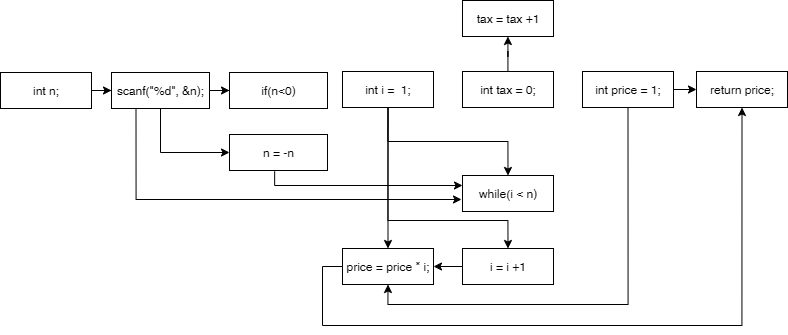
\includegraphics[width = \linewidth]{../images/DDG.png}
    \caption{Data Dependence Graph per il listing 3.2. Adattato da \cite{DDG}}
\end{figure}
\section{Program slicing}
La ricerca di vulnerabilità in software di grandi dimensioni può consumare una grande quantità di tempo e risorse computazionali.
Inoltre, non tutte le computazioni effettuate da un programma sono rilevanti o potenzialmente vulnerabili. 
In questi casi, è possibile ridurre la dimensione dello spazio delle istruzioni da analizzare utilizzando una particolare tecnica di decomposizione
chiamata \textbf{program slicing}.
Questa tecnica produce un nuovo sottoprogramma, denominata \textit{slice}, che include solamente le istruzioni di interesse per una determinata computazione del programma.
Lo slicing di un programma produce il più \textbf{piccolo sottoprogramma eseguibile} che mantiene il comportamento del programma originale rispetto a quella computazione ed è prodotto rispetto ad un \textbf{criterio di slicing}.
Un criterio di slicing è una coppia $C = (V, n)$ dove \cite{Sclicing}:
\begin{itemize}
    \item $V$ è \textbf{l'insieme delle variabili} rilevanti per la computazione di interesse
    \item $n$ è l'insieme dell \textbf{locazioni di interesse} nel programma 
\end{itemize}
Esistono diverse metodologie per effettuare lo slicing di un programma; alcuni esempi sono \cite{Sclicing}::
\begin{itemize}
    \item \textbf{Program slicing statico (Backwards slicing)} Questa tecnica produce uno slice del programma senza tenere in considerazione l'input del programma. Fu la prima tecnica di slicing ad essere presentata \cite{weiser1981program}.
    \item \textbf{Program slicing dinamico}: Proposta da Korel e Laski \cite{korel1988dynamic}, questo tipo di slicing si basa sulla computazione dello slice tenendo in considerazione l'input ricevuto dal programma, il suo percorso di esecuzione e le relazioni di dipendenza tra gli statement.
    \item \textbf{Conditioned slicing}: Questa tecnica funge da ponte tra slicing dinamico e statico. Nel conditioned slicing, una condizione di slicing è una tripla $C_{cond} = (p, V, n)$, dove $p$ è una qualche condizione iniziale di interesse.
\end{itemize}
\newpage \noindent
Proponiamo il seguente esempio: supponiamo di avere il seguente programma e di voler produrre uno slice, utilizzando la tecnica dello \textbf{slicing statico}, rispetto al criterio $(product, 13)$:
\lstinputlisting[language=C, caption = Un programma in C che calcola il fattoriale di un numero $n$ e la somma da $1$ a $n$. Esempio proventiente da \cite{Sclicing}, firstline = 2]{../code_examples/example3.c}
\lstinputlisting[
  language=C,
  caption={{Slice ottenuta applicando slicing statico rispetto al criterio $(product, 13)$}},
  firstline=2
]{../code_examples/slice.c}
\section{Esecuzione simbolica}
Quando avviene la costruzione di un control flow graph per un programma, l'obbiettivo d'interesse è quello di rappresentare tutti i suoi possibili flussi di esecuzione.
Tuttavia, ciò che non viene considerato durante la costruzione di un CFG è l'effettiva praticabilità dei suoi cammini; infatti alcuni cammini presenti sul CFG potrebbero
essere \textbf{irraggiungibili} da un qualsiasi input dato al programma. Possiamo classificare i cammini su un CFG in due diverse categorie:
\begin{itemize}
    \item \textbf{Praticabili} (feasible): Se esiste un input concreto di valore $V$ tale che se il programma è eseguito con $V$, allora esso esegue tutte le istruzioni sul cammino considerato.
    \item \textbf{Impraticabili} (infeasible): Se non esiste nessun input di valore $V$ che porta il programma ad eseguire il cammino considerato. La presenza di cammini non praticabili sul CFG \textbf{non implica necessariamente la presenza di codice morto}, tuttavia la presenza di quest'ultimo implica l'esistenza di cammini non praticabili.
    Spesso, una grossa porzione di tutti i cammini di esecuzione di un programma sono impraticabili.
\end{itemize}
\textbf{L'esecuzione simbolica} funge da ponte tra il comportamento di un programma e la sua logica. 
A differenza dell'esecuzione concreta di un programma, la quale utilizza un input concreto e permette di analizzare solamente un determinato cammino di esecuzione del programma,
l'esecuzione simbolica permette di \textbf{esplorare simultaneamente tutti i cammini praticabili} che il programma potrebbe intraprendere al variare dell'input, eseguendo il programma con valori simbolici \cite{Symbolic_exc_1}.
Un framework di esecuzione simbolica è tendenzialmente composto dalle seguenti componenti \cite{Symbolic_exc_1}:
\begin{enumerate}
    \item \textbf{Esecutore simbolico}: Esegue il programma utilizzando input simbolici. Per ogni cammino di esecuzione esplorato, mantiene le seguenti informazioni:
    \begin{itemize}
        \item \textbf{Path condition}: Una formula booleana nella logica del primo ordine che caratterizza lo stato d'esecuzione del programma. Essa esprime, sotto forma di vincoli logici, le condizioni soddisfatte dall'input durante l'esecuzione simbolica del programma.
        Ogni istruzione di branch che viene eseguita dall'esecutore aggiorna la path condition per un determinato cammino con un nuovo vincolo. 
        \item \textbf{Memoria simbolica}: Mappa le variabili a delle espressioni o valori simbolici. Le istruzioni di assegnamento del programma aggiornano la memoria simbolica dell'esecutore.
    \end{itemize}
    \item \textbf{Model checker}: Un model checker, tipicamente un \textit{Satisfiability modulo theories} (SMT) solver, viene utilizzato per controllare se vi sono delle violazioni logiche nella path condition rispetto ad una proprietà d'interesse (per esempio, una proprietà di sicurezza) e se il cammino è praticabile, cioè se la path condition che
    lo caratterizza è una formula \textbf{soddisfacibile}. In generale, il problema della soddisfacibilità booleana (conosciuto con il nome di SAT) è un problema \textbf{indecidibile}; tuttavia, può essere risolto in un gran numero di casi pratici; per esempio, 
    i vincoli booleani lineari (es. $X > Y \land X + Y \leq 10$) sono spesso risolubili in maniera efficiente.
\end{enumerate}
L'esecuzione simbolica di un programma può, inoltre, avvenire in due diversi modi:
\begin{itemize}
    \item \textbf{Esecuzione simbolica statica}: L'esecuzione avviene senza effettivamente eseguire il programma. Vengono esplorati tutti i possibili cammini praticabili del CFG.
    \item \textbf{Esecuzione simbolica dinamica (analisi concolica)}: l'esecuzione simbolica del programma viene affiancata ad un'esecuzione; vengono quindi esplorati ed eseguiti simbolicamente solo i cammini raggiunti dal valore concreto dell'input.
\end{itemize}
Supponiamo, per esempio, di voler eseguire simbolicamente (in maniera statica) il seguente programma:
\lstinputlisting[
  language=C,
  caption={{Un programma in C che controlla se l'utente ha scritto un numero tra cinque e sette}},
  firstline=2
]{../code_examples/example4.c}
L'esecutore simbolico esplorerà tutti i cammini praticabili del programma:
\begin{itemize}
    \item \textbf{Variabili simboliche}: $x = X$ con $X$ valore simbolico
    \item \textbf{Path condition}:
    \begin{itemize}
        \item \textbf{Percorso A}: $X >= 5 \land X <= 7$
        \item \textbf{Percorso B}: $X < 5 \vee X > 7$
    \end{itemize}
\end{itemize}
\section{Disassembling}
Generalmente, la catena di compilazione di un linguaggio ad alto livello prevede una fase di \textit{assemblaggio}, in cui il codice assembly generato dal compilatore viene tradotto
nel linguaggio macchina specifico dell'architettura della CPU su cui il programma dovrà essere eseguito. Questa traduzione stabilisce quindi una relazione uno-a-uno tra le istruzioni macchina
prodotte dall'\textit{assemblatore} e le istruzioni assembly definita dalla \textit{Instruction Set Architecture} (ISA) dell'architettura del processore.
Questa relazione permette di effettuare anche la traduzione inversa e recuperare il codice assembly dall'insieme di istruzioni macchina presenti in un file binario.
Questo processo è noto con il nome di \textbf{disassembling}. Effettuare il disassembly di un programma è una pratica fondamentale nell'ambito del reverse engineering, poiché permette di analizzare, in un formato leggibile dall'essere umano (assembly), le operazioni
di basso livello che verranno eseguite dal calcolatore, rendendo possibile l'individuazione di potenziali problematiche di sicurezza sfruttabili da un attaccante.
Seppur sembri un processo relativamente semplice, effettuare il disassembly di un codice macchina richiede di gestire diverse problematiche \cite{Disassembly2}:
\begin{itemize}
    \item \textbf{Jump tables}: una \textit{jump-table} è un array di indirizzi comunemente usata per per implementare trasferimenti del flusso di controllo multi-direzionali (ad esempio, la trasposizione a basso livello del costrutto \textit{switch} del linguaggio \textit{C}).
    L'idea alla base dell'utilizzo di una jump table è quella di recuperare l'indirizzo a cui saltare indicizzando l'array con il valore dell'espressione per poi effettuare un jump indiretto verso l'indirizzo recuperato.
    Il codice che si occupa di questo processo è di solito preceduto da un controllo sul valore dell'espressione (\textit{bound check}) per assicurarsi che non si stia cercando di accedere ad un indice non presente nell'array.
    Un disassembler dovrà quindi necessariamente stimare correttamente la grandezza della jump table per garantire la qualità del disassembly prodotto.
    \item \textbf{Position-Independent Code (PIC)}: Molti compilatori generano codice che può essere caricato ed eseguito indipendentemente dalla specifica sezione dello spazio di indirizzamento in cui vene caricato il programma.
    Questo tipo di codice viene detto \textit{Position-Independent Code} (PIC). Quando viene prodotto PIC, il compilatore tipicamente crea delle \textit{jump tables}, anch'esse indipendenti dalla posizione e formate da una serie di offset, le quali vengono inserite all'interno della sezione dell'eseguibile dedicata al codice (la "\textit{text}" section).
    L'offset presente all'interno di queste tabelle verrà poi sommato all'indirizzo caricato al momento pe raggiungere la posizione desiderata tramite un jump indiretto.
    La presenza di PIC introduce due criticità che complicano il processo di disassembly:
    \begin{itemize}
        \item Le tabelle sono \textbf{indistinguibili dai dati presenti nell'eseguibile}
        \item Le sezioni di codice che effettuano i jump indiretti sono spesso \textbf{complesse} e non aderiscono a pattern di codice facilmente riconoscibili
    \end{itemize}
    Considerate insieme, queste caratteristiche rendono il disassembly di sequenze di PIC contenenti jump table più problematiche rispetto all'analisi di codice standard.
\end{itemize}
\section{Decompiling}
Dato un programma binario, è possibile \textbf{ricostruire il codice ad alto livello} in cui è stato scritto attraverso un processo noto come \textit{decompiling}.
Lo scopo di un \textit{decompiler} (o \textit{reverse compiler}) è quindi quello di recuperare, partendo dal codice macchina, un programma scritto in un linguaggio ad alto livello che effettua le stesse
operazioni del programma binario dato in input \cite{Cifuentes1995DecompilationOB}.








\end{document}